\chapter{Úvod}

\todo{reference na kapitoly ..ref..}

1) 5 radku obecny uvod
Zpracování řeči hraje v dnešní době důležitou roli v mnoha rozličných oborech. Mezi jedny z hlavních úkolů bezesporu patří separace zdrojů v nějakém zaznamenaném signálu, který může být složen ze signálů N mluvčích, ale i nechtěnému hluku okolí. Vyřešení problému je předpoklad k dalším úkonům jako identifikace konkrétního mluvčího nebo třeba přepis mluveného slova na text. Se stále se zrychlujícím vývojem počítačů a s jejich zvyšujícím se výkonem se do popředí dostávají metody zpracování řeči založené na neuronových sítích, které v mnoha ohledech předčily doposud používané algoritmy.

2) proc je prace v dane oblasti dulezita, vyznam pro svet a pro nas
Separace mluvčích v časové doméně dosahuje mimořádných výsledků v porovnání s dosavadními metodami LSTM založenými na převodu signálu z časové domény do frekvenční domény. Taková reprezentace signálu není optimální pro udržení časových závislostí, které jsou při zpracování řeči podstatné. V referenční studii je vstupní signál převeden do nezáporné reprezentace, která je optimální pro extrakci jednotlivých mluvčích. Silnou stránkou systému je hluboká architektura sítě, která dokáže zachovat dlouhodobé závislosti v signálu.

3) o minulosti, stav dnes a vyhlidky do budoucna


4) proc se tematu chci venovat, proc je podle me perspektivni = motivace
Téma v oblasti neuronových sítí jsem si vybral, jelikož ty zažívají obrovský rozmach a pomalu se stávají součástí téměř všech odvětví.
\todo{nejak to jeste dopsat tohle.}


5) co je cilem me prace - vlastnimi slovy
Má práce si klade za cíl implementovat neuronovu síť podle architektury TasNet pro separaci mluvčích, která byla navržena a popsána ve studii\ref{referencni_studie}. Následně tuto neuronovou síť natrénovat s různými kombinacemi hodnot hyperparametrů ovlivňujících velikost sítě a její vlastnosti a nakonec porovnat přesnost mezi jednotlivými sitěmi a mezi výsledky studie. Přesnost separace je vypočítána za pomoci míry si--snr, udávající poměr mezi chtěným signálem a hlukem na pozadí.
\todo{reference na sisnr na wiki nebo v nejake studii???}


6) struktura prace - popsat kapitoly
\todo{prepsat podle novejch kapitol co jsem navrhoval - doplnit popsani datasetu}
V první části práce jsou popsány základní prvky neuronových sítí, struktura umělého neuronu, jeho vstupy a výstupy, váhy a role aktivační funkce. V návaznosti na to je popsán proces učení neuronové sítě. Ten se skládá z několika souvisejících částí, které zahrnují výpočet výstupu neuronové sítě metodou feed forward, který transformuje vstupní hodnoty a počítá na základě nich výstup, který propaguje do dalších vrstev neuronové sítě. Dále je rozebrán výpočet chyby, která vzniká během procesu učení, metodou gradient descent a nakonec úprava vah neuronů metodou backpropagation, která se počítá na základě rozdílu mezi vstupními hodnotami a očekávánými výstupními hodnotami.

Předtím, než jsou představeny konvoluční sítě, tak je vysvětlena samotná konvoluce.
Dále je vysvětlen princip konvolučních neuronových sítí, které se používají nejčastěji pro zpracování obrazu kvůli vlastnostem, které umožňují extrahovat příznaky s různou úrovní složitosti od základních útvarů jako úsečka, barva a podobně až po například část obličeje -- ucho, nos, či úplně celý obličej. Tohoto lze využít i při zpracování zvuku, kde jsou tyto extrahované příznaky jednorozměrné.

Se znalostí principu konvolučních sítí je představen konvoluční auto-enkodér, který převádí vstupní nahrávku směsi mluvčích na reprezentaci optimalizovanou pro separaci jednotlivých mluvčích.

Druhá část je věnována architektuře TasNet. V této kapitole je popsána podoba separačního modulu, jeho stavební bloky a princip. Postupně je znovu zmíněn konvoluční auto-enkodér, u nějž je vysvětlen jeho úkol v separačním modulu a následně konvoluční blok, který se sám sestává z konvolučních vrstev, normalizací a aktivačních funkcí. Tyto bloky jsou skládány za sebe se zvyšující se časovou dilatací a tvoří jádro separačního modulu.

Třetí část se zabývá implementací neuronové sítě. Je popsán a odůvodněn zvolený framework pytorch, využité prostředky a metody.
\todo{nejak to jeste dopsat tohle.}

Na závěr jsou popsány experimenty s modelem - rychlost učení, vliv hyper-parametrů na učení sítě, na výsledky a přesnost výstupu v závislosti na zvolených parametrech, optimalizacích a počtu konvolučních bloků a pod. Výstup sítě v podobě separovaných mluvčích je porovnán s referenční studií.
\todo{Zminit zde taky sisnr hodnoceni a pod.}

%----------------------------------------------------------------------------------------------------------------------------------------------------------------------
\todo {Teorie: Co bylo potreba nastudovat;; uvod do problematiky;; pisu to pro nekoho, kdo chce vychazet z me bakalarky.}

\chapter{Separace mluvčích}
\label{separacemluvcich}
- obecne o problemu separace; prostredi a vyuziti, coctail party, multispeech

\chapter{Neuronové sítě}
\label{neuronovky}
body: co vlastne resi . skladaji se ze vstupni vrstvy, N skrytych vrstev, vystupni vrstvy
Co resi neuronove site.

V dnešní době zažívají neuronové sítě díky výkonosti počítačů velký rozmach. Jejich využití prostupuje skrze mnohé vědní obory a nově dokáže řešit celou řadu problémů, ve kterých dosahuje výborných výsledků, které zdaleka předčily dosavadní postupy. Mezi nejčastější úlohy, na které se neuronové sítě používají, jsou klasifikační úlohy, rozpoznávání obrazu a řeči či vzorů na videu nebo ve zvuku až po generování textu. Na základně řešeného problému vzniklo mnoho druhů neuronových sítí, z nichž některé zde budou představeny.

Nejzákladnější neuronová síť je vícevrstvá neuronová síť, neboli MLP (Multi Layer Perceptron). Tento typ sítě je skládá ze třech typů vrstev. Vstupní vrstva slouží k předání hodnot do sítě. Tato vrstva nijak nemodifikuje vstupní hodnoty, které jsou do sítě předávány a nezměněné je kopíruje první skryté vrstvě. Každá vrstva se může skládat z $1$ až $N$ neuronů, kde $N \in N$. Poslední skrytá vrstva je napojena na výstupní vrstvu. Výstupní vrstva má obvykle méně neuronů než předešlé vrstvy a hodnoty na výstupu mohou představovat třídy, do kterých má být zařazen vstup. S počtem jednotlivých vrstev souvisí pojem hloubka sítě, která je rovna počtu všech vrstev neuronové sítě od vstupní až po výstupní vrstvu.

Takto propojené neurony tvoří acyklický graf, který počítá a následně předává hodnoty směrem od vstupní vrstvy skrze skryté vrstvy až k vrstvě výstupní. Nenacházejí se zde žádná zpětná spojení, ve kterých by se výstup vracel zpět do sítě.\cite{mitdeeplearning}

Cílem takové neuronové sítě je aproximovat nějakou funkci $f^\ast$. Síti je předána vstupní hodnota $x$ a výstupní hodnota $y^\ast = f^\ast(x)$ má být co nejblíž hodnotě $y = f(x)$.


\section{Umělý neuron}
Základní stavební jednotka neuronových sítí je neuron, nebo přesněji perceptron. Tento model je založen na reálných poznatcích o neuronech, které se nacházejí v organizmu. Perceptron obsahuje libovolně mnoho vstupních synapsí, přes které se neuronu předá vstupní hodnota, váhy a jeden výstup, jehož hodnota závisí na vstupních hodnotách, vnitřním stavu neuronu (hodnoty vah a biase) a zvolené aktivační funkci. Vstupní hodnoty jsou váhovány, což v praxi znamená, že každá vstupní hodnota je vynásobena s váhou daného vstupu. Váhy v perceptronu představují nějaký vektor vah $w = [w_1, w_2, \dots, w_n]$, se kterým je vynásobený vektor vstupních hodnot $x = [x_1, x_2, \dots, x_n]$.

\todo{obrazek neuronu a popis}
\begin{figure}[H]
    \centering
    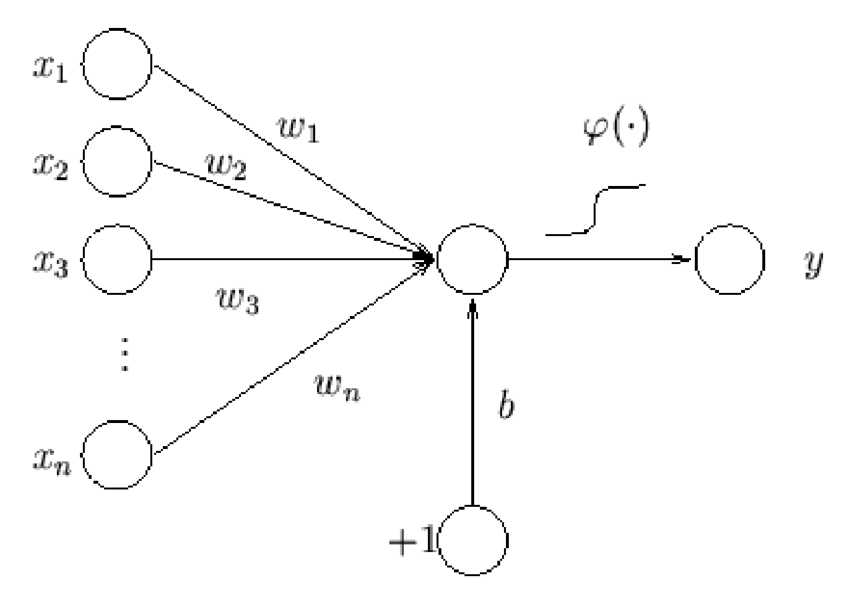
\includegraphics[scale=0.5]{obrazky-figures/perceptron.png}
    \caption{\label{fig:neuron}Schéma umělého neuronu -- perceptron}
\end{figure}

Hodnota bias $b \in R$, která je přičtena k sumě násobků vah a vstupních hodnot, modifikuje dobu, kdy se aktivuje perceptron a změní svůj výstup. Je to prahová hodnota, na základě níž je měněn výstup. Matematicky to znamená, že s aktivační funkcí horizontálně pohybuje doleva nebo doprava v závislosti na tom, je-li bias pozitivní nebo negativní. Bias se učí zároveň s ostatními váhami během učícího procesu.

\begin{figure}[H]
    \centering
    
\includegraphics[scale=1]{obrazky-figures/placeholder.pdf}
    \caption{\label{fig:bias}Vliv hodnoty bias na aktivační funkci}
\end{figure}

Výstup neuronu se vypočítá jako:
\begin{equation}
y = a((\sum_{n=1} w_nx_n) + b)
\end{equation}
kde $a$ je nějaká aktivační funkce, $x_n \in R$ je vstupní hodnota, $w_n \in R$ je váha, kterou se vstupní hodnota vynásobí a $b \in R$ je hodnota bias, která je přičtena k celkové sumě předtím, než se výsledek předá aktivační funkci.


\section{Aktivační funkce}
Aktivační, neboli prahová funkce určuje výstupní hodnotu neuronu. Funkce se vybírá na základě problému, který se má neuronová síť naučit řešit. Správná volba prahové funkce vede k lepší konvergenci učení sítě. Naopak špatná volba může vést ke stále větší odchylce od správného řešení -- může divergovat. Povaha problému může vyžadovat specifické vlastnosti aktivační funkce - lineární nebo nelineární -- sigmoidní a podobně. Pro správnou volbu aktivační funkce je pro nestandardní problémy potřeba experimentálně zjistit, která bude nejlépe vyhovovat.

\subsection*{Sigmoid}
\begin{equation}
  f(x) = \frac{1}{1+\exp(-z)}
\end{equation}
\blindtext{1}
\begin{figure}[H]
    \centering
    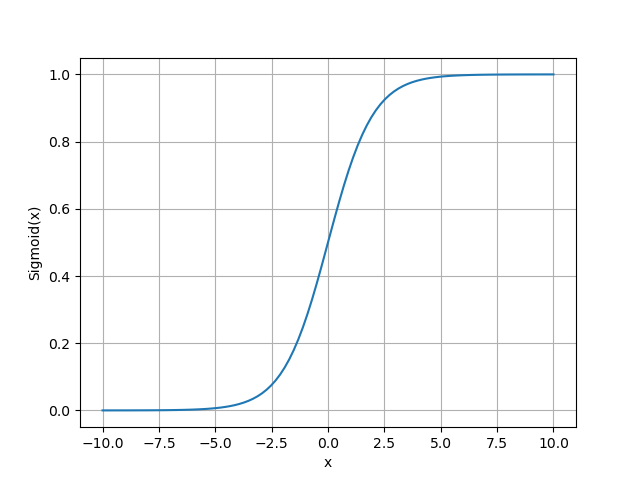
\includegraphics[scale=0.2]{obrazky-figures/sigmoid.png}
    \caption{\label{fig:sigmoid}Graf aktivační funkce sigmoid}
\end{figure}

\subsection*{Softmax}
\begin{equation}
  f(x) = \frac{1}{1+\exp(-z)}
\end{equation}
\blindtext{1}
\begin{figure}[H]
    \centering
    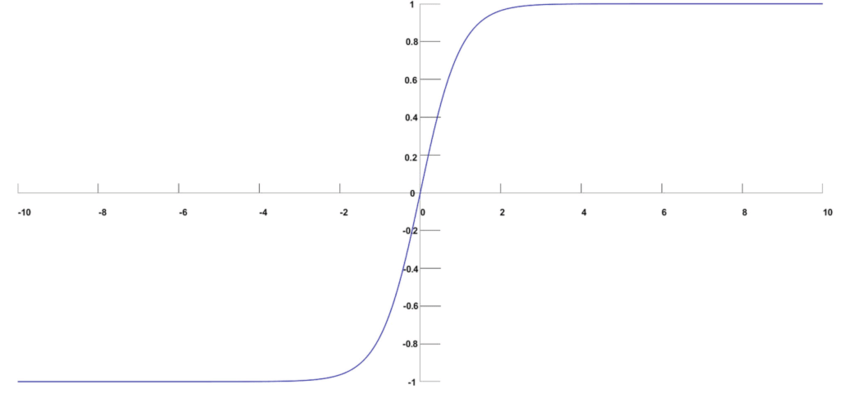
\includegraphics[scale=0.2]{obrazky-figures/softmax.png}
    \caption{\label{fig:softmax}Graf aktivační funkce softmax}
\end{figure}

\subsection*{ReLU}
Rectified Linear Unit je nejčastěji používaná aktivační funkce. Vyžaduje-li neuronová síť nějakou nelinearitu, je RelU pro většinu případů ideální. Pro každou zápornou hodnotu $x$ vrací $0$ a pro kladnou hodnotu $x$ vrací tutéž hodnotu $x$.
\begin{equation}
   f(x)=max(0,x)
\end{equation}
\blindtext{1}
\begin{figure}[H]
    \centering
    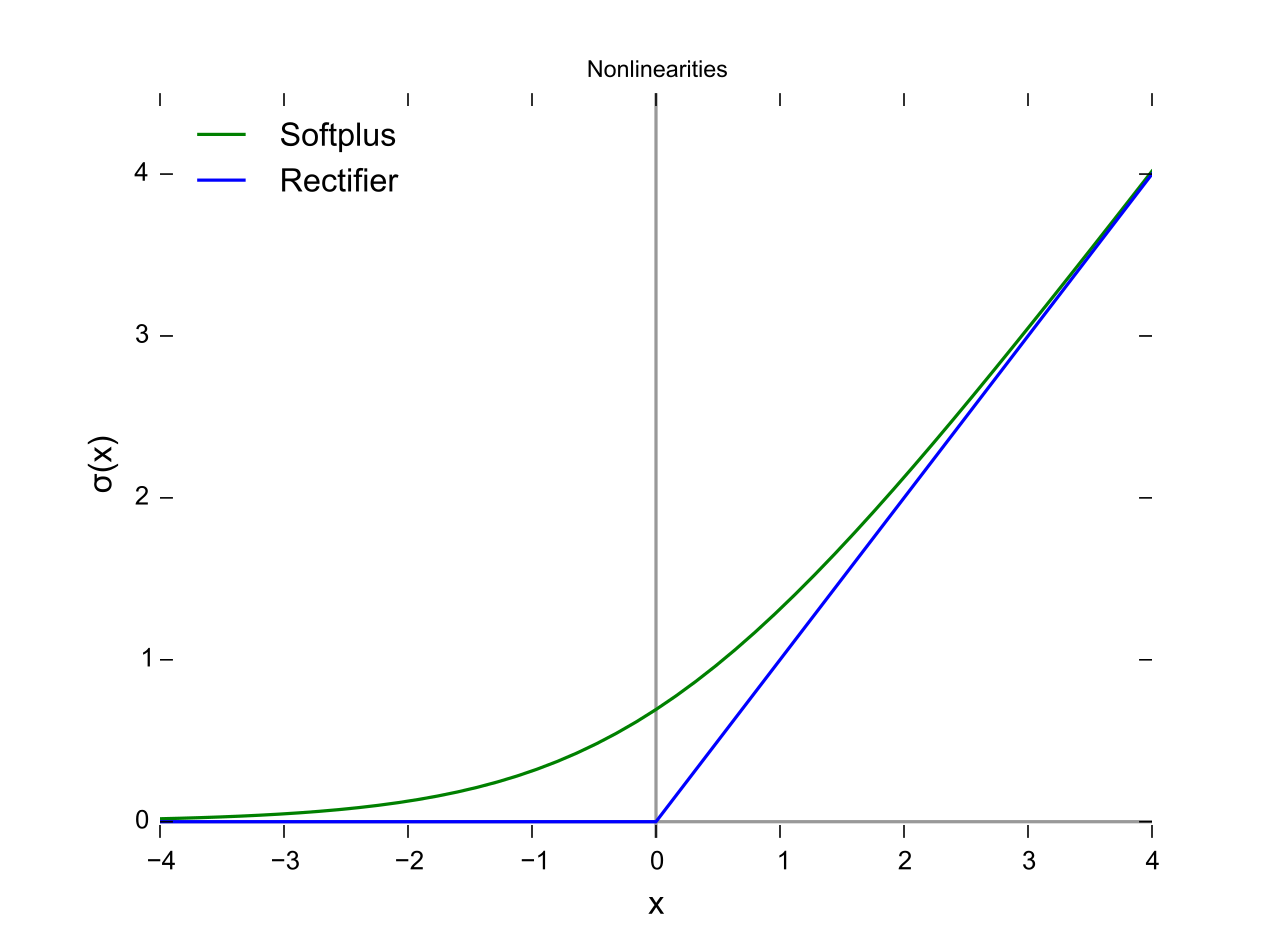
\includegraphics[scale=0.2]{obrazky-figures/ReLU.png}
    \caption{\label{fig:relu}Graf aktivační funkce ReLU}
\end{figure}


\subsection*{PReLU}
Parametrizovaná ReLU je nelineární aktivační funkce, která se používá v případě, že chceme produkovat na výstup malý nenulový gradient i v případě záporné vstupní hodnoty $x$. V tom případě je vstupní hodnota vynásobena parametrem $\alpha$ a to představuje výsledek. Parametr $\alpha$ se společně s ostatními váhami učí během učícího procesu.
\begin{equation}
  f(x) =
  \begin{cases}
    x & \text{if } x \geq 0 \\
    {\alpha}x & \text{if } x < 0
  \end{cases}
\end{equation}
\blindtext{1}
\begin{figure}[H]
    \centering
    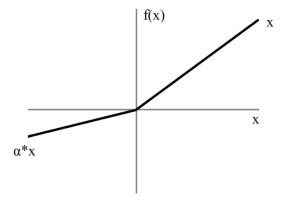
\includegraphics[scale=1]{obrazky-figures/prelu.jpg}
    \caption{\label{fig:prelu}Graf aktivační funkce PReLU}
\end{figure}



\section{Proces učení neuronových sítí}
\blindtext{1}

\subsection{Objektivní funkce}
= cost funkce
-popis, co to je, k cemu to je, proc to je...

\subsection*{MSELoss}
- vzorecek
\subsection*{Cross Entrophy}
- vzorecek

\subsection{Inicializace parametrů}
\todo{Mozna, Kniha strana 292}


\subsection{Optimalizační algoritmy}
 [1 deep learning str 301]

\subsection*{Adam}

\todo{Kniha strana 301}

Adam je jeden z algoritmů s adaptivním učením. Jeho název byl odvozen z fráze "adaptive moments".  [1 deep learning str 301]


\subsection{Backpropagation}
- zpetne sireni chyby
- adaptacni algoritmus, podil neuronu na chybe,
- 3 opakujici se faze uceni:

\todo{dodelat zde podkapitoly v lepsim poradi}

1) feedforward - dopredu
2) zpetne sireni chyby - Backpropagation
3) uprava vah a biasu na zaklade chyby
- chain rule

\blindtext{1}


\subsection*{Feed Forward}
\blindtext{1}

\subsection*{Gradient descent}
\blindtext{1}

\subsection{Overfitting a generalizace}
\blindtext{1}


\section{Konvoluční neuronové sítě}
\blindtext{1}

\subsection{Konvoluce}
\blindtext{1}


%----------------------------------------------------------------------------------------------------------------------------------------------------------------------


\chapter{TasNet - Time--Domain Audio Separation Network}
\label{tasnet}
\todo{Architektura full -- obrázek, bloky...}
\begin{figure}[H]
    \centering
    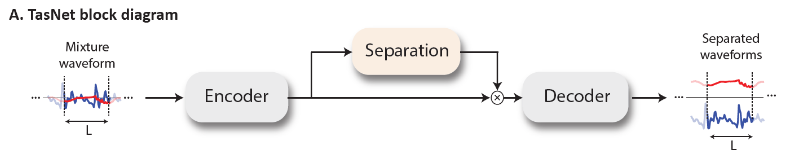
\includegraphics[scale=0.5]{obrazky-figures/tasnet-pipe.png}
    \caption{\label{fig:tasnet-pipe}Zjednodušený model architektury}
\end{figure}
\blindtext{1}

\section{Konvoluční auto--enkodér}
\todo{Konvoluční autoenkodér, vstup, výstup...}

- schema bez separacniho modulu
- non negative representation of audio
\begin{figure}[H]
    \centering
    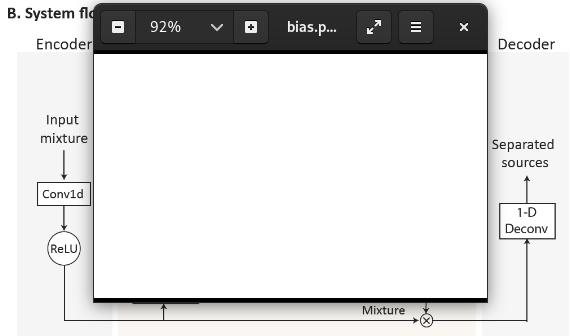
\includegraphics[scale=0.5]{obrazky-figures/tasnet-autoencoder.png}
    \caption{\label{fig:tasnet-autoencoder}Schéma konvolučního autoenkodéru}
\end{figure}
\blindtext{1}

\section{Separační modul}
- odhad masek pro jednotlive mluvci
- schema se separacnim modulem
\begin{figure}[H]
    \centering
    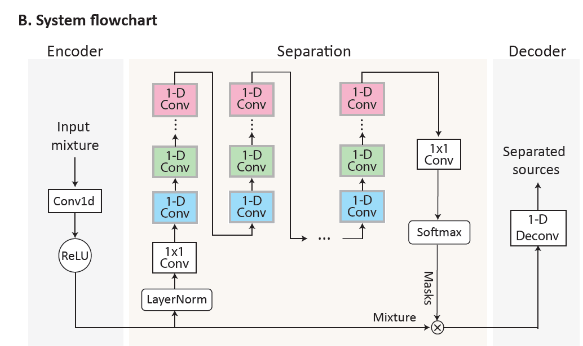
\includegraphics[scale=0.6]{obrazky-figures/tasnet-architecture.png}
    \caption{\label{fig:tasnet-modul}Schéma architektury TasNet}
\end{figure}

\blindtext{1}

\subsection{Konvoluční bloky}
- Z čeho se skládá -- konvoluční vrstvy, normalizace
- diagram konv bloku.
- Mozna: Dilatace a time perception
\begin{figure}[H]
    \centering
    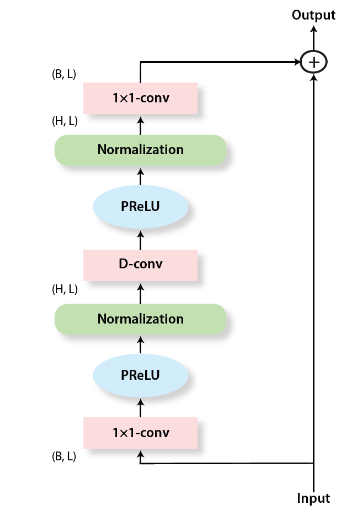
\includegraphics[scale=0.5]{obrazky-figures/conv-res-block.png}
    \caption{\label{fig:tasnet-convblock}Jeden konvoluční blok}
\end{figure}

\blindtext{1}

%----------------------------------------------------------------------------------------------------------------------------------------------------------------------



\chapter{Implementace a trénování sítě}
\label{implementace}
Pozn: colab, pytorch, stroj, bash, hyperparams, vykon a cas trenovani, seg--len, popis trid.

\section{Dataset}
\todo{Ukazat zde vykreslenou vlnu nahravek mix, s1, s2}
\todo{popsat co je dataset a k cemu to slouzi}
Trénování a vyhodnocení modelu proběhlo na množině jednokanálových nahrávek směsí dvou mluvčích. Množina byla vygenerována náhodným výběrem různých mluvčích z Wall Street Journal (WSJ0) a vytvořením směsi. Celková délka trénovacích dat je přes 10 hodin a přes 6 hodin validačních dat. Nahrávky jsou převzorkovány na 8kHz a během trénování zarovnány na zero means a jednotkovou varianci[studie str 5 Dataset][49 - ze studie odkaz na script na generovani a popis na netu].
\todo{doplnit info o zero means a jendotkove varianci}

\subsection{Význam validační množiny v trénování}
Většina algoritmů strojového učení má nějakou sadu hyperparametrů, kterou je upravováno chování algoritmu. Hodnoty hyperparametrů obvykle bývají nastavovány ručně ještě před spuštěním procesu učení a hodnota se v průběhu nemění, protože hodnoty by bylo obtížné optimalizovat. 
Některá nastavení se nicméně mohou stát hyperparametrem a být upravována během trénování, ale není vhodné je měnit na základě výsledku učení na trénovací sadě, protože by mohlo dojít k přetrénováníoverfitting) v důsledku \todo{CEHO??}. Pro tento případ potřebujeme validační sadu, která je odlišná od trénovací sady.
Po každém zpracování trénovací sady následuje validační sada, po jejímž skončení jsou optimalizovány hyperparametry[][].
\begin{figure}[H]
    \centering
    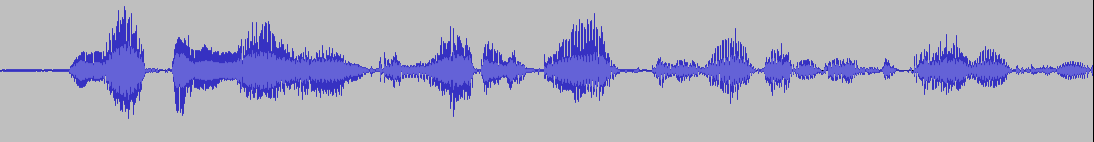
\includegraphics[scale=0.35]{obrazky-figures/dataset-mix.png}
    \caption{\label{fig:ref-mixture}Ukázka nahrávky směsi dvou mluvčích}
\end{figure}
\begin{figure}[H]
    \centering
    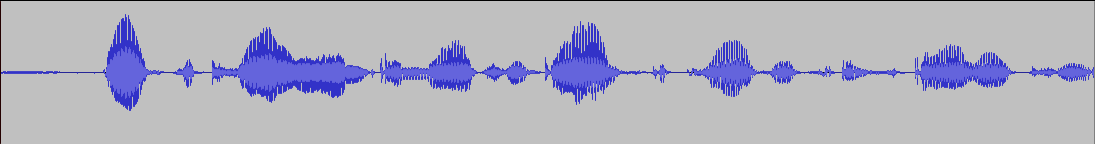
\includegraphics[scale=0.35]{obrazky-figures/dataset-s1.png}
    \caption{\label{fig:ref-s1}První mluvčí ze směsi}
\end{figure}
\begin{figure}[H]
    \centering
    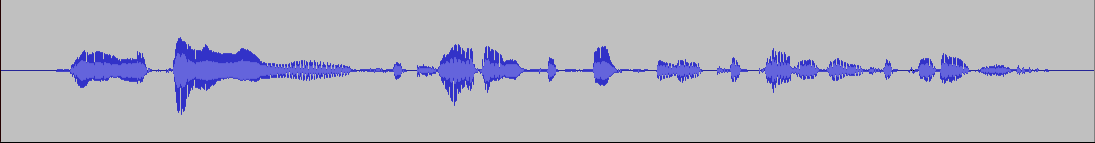
\includegraphics[scale=0.35]{obrazky-figures/dataset-s2.png}
    \caption{\label{fig:ref-s2}Druhý mluvčí ze směsi}
\end{figure}
Lze si všimnout, že sečtením signálů separovaných mluvčích na obrázku (ref obr1) a obrázku (ref obr2) dostaneme přesně signál směsi, což lze vyjádřit vztahem
\begin{equation}
  x(t) = \sum_{i=1}^C s_i(t)
\end{equation}
, kde $x(t) \in R^{1 \times T}$ je diskrétní signál směsi a $s_i(t) \in \mathbb{R}^{1 \times T}$, kde $i = 1,\ldots,C$, je jeden z $C$ zdrojů[ref studie str3 vlevo]. 
\todo{[kniha 117-118] kap 5.3 = Hyperparameters and validation set} 
\todo{najit jeste nejakej zdroj s popisem a pripadne nejaky zajimavejsi info.}

\section{Vyhodnocovací metriky}
- minimalizovat objektivni-hodnotici funkci sisnr.
\subsection{Signal to noise ration}
\subsection*{Source Distortion Ratio -- SDR}
\subsection*{Artifacts Ratio -- SAR}
\subsection*{Inference Ratio -- SIR}

\subsection{Implementace modelu}
- pytorch, scripty, python3, bash, tridy, moduly, parametry a volby spusteni.

%----------------------------------------------------------------------------------------------------------------------------------------------------------------------


\chapter{Experimenty a vyhodnocení}
\label{experimenty}
- trenovani s ruznymi hyperparametry, uspesnost a tabulky s hyper parametry a dosazenymi vysledky a hodnotami sisnr, sdr atd.
- model size comparison.
- porovnani s vysledky ze studie
- obrazky separovanych mluvcich - signalu.
- spektra
- grafy trenovani loss a vysledkuu.
- pametova narocnost modelu


\section{Možná rozšíření a navrhnutá vylepšení}
- variabilnější dataset, mikrofony, šum a bordel prostředí
- separace více mluvčích
- hlučné prostředí
- identifikace konkrétního řečníka
- realtime separace

%----------------------------------------------------------------------------------------------------------------------------------------------------------------------

\chapter{Závěr}
\label{zaver}
- co jak dopadlo, vysledky a vyhodnoceni velikosti modelu a jaky byl nejlepsi,...
\blindtext[3]

